\documentclass{article}
\usepackage{amsmath}
\usepackage{gensymb}
\usepackage{parskip}
\usepackage[none]{hyphenat}

\usepackage[margin=1in, left=1.5in, includefoot]{geometry} 


%graphic stuff

\usepackage{graphicx} % allows images

\usepackage{float} %helps with posisioning


%header and footer stuff

\usepackage{fancyhdr}

\pagestyle{fancy}

\fancyhead{}

\fancyfoot{}

\fancyhead[L]{Robotic Artist:Walter / 0.3.1 (WIP)}

\fancyfoot[L]{Aberystwyth University / Computer Science}

\fancyfoot[R]{page: \thepage}

\renewcommand{\headrulewidth}{0pt}

\renewcommand{\footrulewidth}{0pt}


%begins document

 \begin{document}



    % begin title screen

    \begin{titlepage}

        \begin{center}

        \line(1,0){340}\\ 


        \large{\bfseries Robotic Artist:Walter} \\

        \large {\bfseries G400 Computer Science, CS39440 }\\
        
        \large {\bfseries Design Specification}\\


         \line(1,0){250}\\

         \textsf {Author: Matthew Howard \\
          Candidate Number: 150035512\\
          User ID: Mah60 \\
          Supervisor Name: Helen Miles \\
          Supervisor ID: Hem23\\
          Last Modified: 27/04/2018 \\
          Version: 0.3.1\\
          Status: Work In Progress(WIP)} \\

        \end{center}        

    \end{titlepage}
  
    \clearpage

     \tableofcontents
     
     \clearpage

    \section{Introduction}
This document is going to define the overall design of the product as a whole. It describes the structure of the product and how it maintains the integrity of the design.\\ \newline
The Design specifications will include version control and the UML diagrams that describe the structure of the product that has been developed. This includes UML diagrams for sequences and class layouts to describe dynamic and static views of the design. 
\\ \newline
The design that has been developed must meet the requirements within the Requirement Specifications.\cite{Requirement_specifications}
    \section{Version Control}
Version control is maintained in this project through a Github Repository. Github stores  different versions of the code that have been committed to the repository as the project has progressed. Github also allows for branches to be made in which you can try out new versons of code and decide when to implement it to the master version of the product stored on Github.\\ \newline
Github has been used in this project to maintain different versions of the code and could be used to backtrack the code if there are major errors or faults in the project.
\\ \newline
Another, form of version control within the code and documentation is that at the top of every module and the end of the document there is a version history section. This talks about what has been done to modify the document and why it has been done in a clear way and the date that this modification was done. An example of this can be seen in Figure \ref{fig:Version_Control}.

\begin{figure}[h]
    \centering
    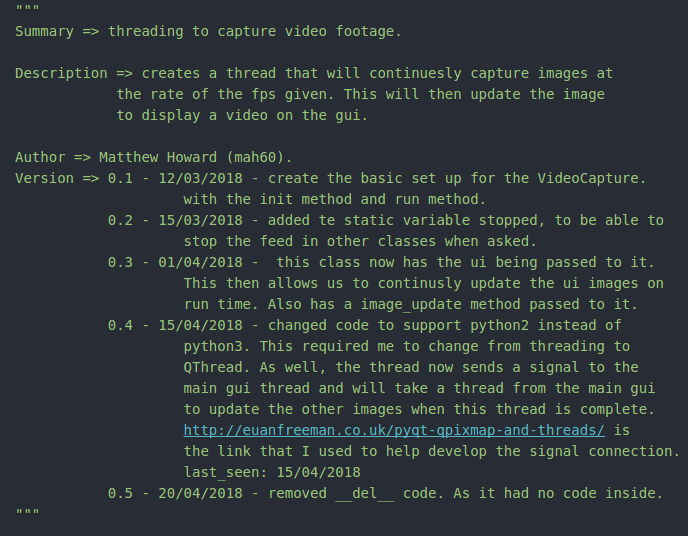
\includegraphics[width=0.5\textwidth]{version_control.png}
    \caption{Demonstrates the Version control that is being used in the video\_capture.py Module. This includes the version number, description and date of change.}
    \label{fig:Version_Control}
\end{figure}
\clearpage
    \section{UML Diagrams}
In this section of the design specifications, the document describes the framework of the code, how the code is structured and runs on real-time events that occur. This will be done by using UML diagrams. 
\subsection{Class Diagram} 
\begin{figure}[h]
    \centering
    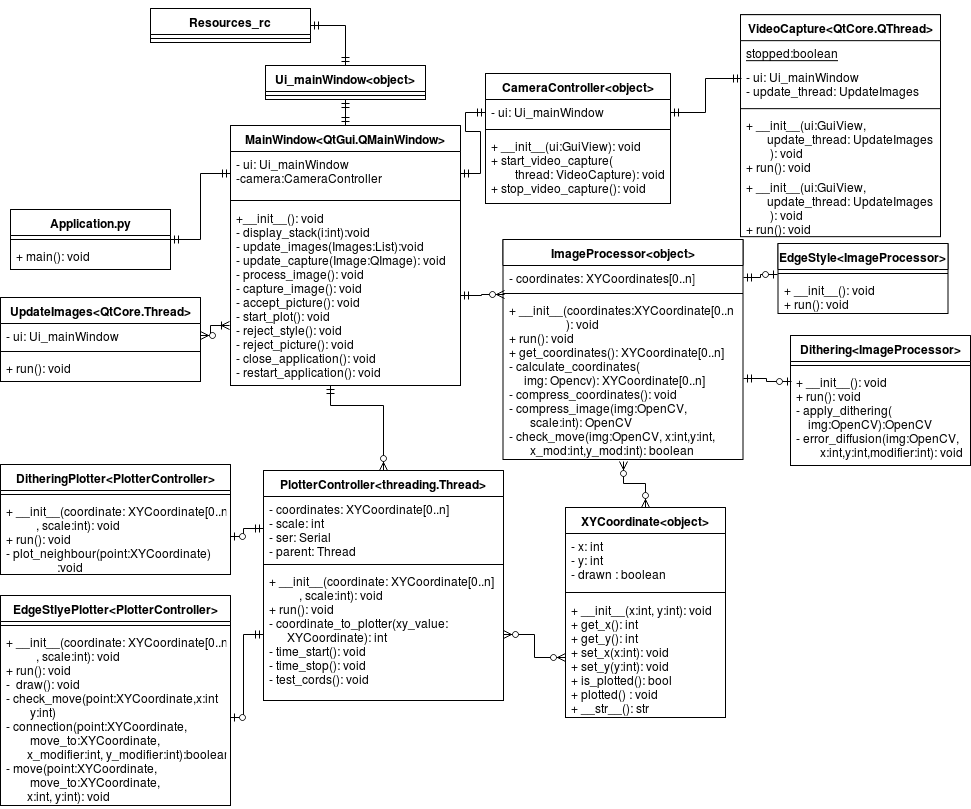
\includegraphics[width=1\textwidth]{class_diagram.png}
    \caption{Displays the UML class diagram. This is the structure of all the classes in the products code.}
    \label{fig:class_diagram}
\end{figure}
Figure \ref{fig:class_diagram} describes the structure of the code that has been developed. The structure of the code has been developed around the MainWindow class, which is the code for controlling the graphical unit interface(GUI). This code is connected to the Ui\_Mainwindow, which is a set of code that has been developed from the QT Designer software\cite{qt_designer}. This allowed the overall framework for the GUI to be developed using various tools within the software.\\ \newline
After this there are three major sections to the class diagram(Figure \ref{fig:class_diagram}). These are the Camera, Image Processor, and the PlotterController.
\\ \newline
The CameraController controls the inputs and outputs from the camera. The VideoCapture is the main thing the controller works with. This is done by creating a thread that continuously sends frames to the GUI to be updated. Once the method stop\_video\_capture is called, then the video capture is stopped and the picture is taken from the frame that the thread was on at that time. The sequence of events can be seen in Figure \ref{fig:SD_video_feed}. The thread is stopped by there being a static variable within the VideoCapture class called 'stopped', this variable is a boolean. This is changed to True when the video thread should be stopped and to False when the capture is running. \\ \newline
The next sections of the class diagram are the ImageProcessor classes. The ImageProcessor class will be a parent to all the styles that are developed for this program. The code that is generated for this class will be used over all the individual ImageProcessors. The main requirements of each style is that they will require a partner PlotterController to plot the final output and an output of coordinates to be plotted. This is where the XYCoordinate class is used to create a generic structure to translate data between the two classes. The XYCoordinate stores x,y values of points to be plotted. As well, a boolean that determines whether the point has been plotted or not.\\ \newline
Finally, we have the PlotterConroller which is a parent class to all plotters for their specific style. The PlotterController will contain code that is generic to all styles plotting routines. An example of this is the coordinate\_to\_plotter() method which will translate coordinate values to plotter values. The overview of the plotter requirements is that it must send serial commands in HPGL to the plotter, to plot out the specified style for that plotter controller.
\\ \newline
\subsection{Sequence Diagrams}
Figures \ref{fig:SD_video_feed}, \ref{fig:SD_image_processing} and \ref{fig:SD_plotting} describe the sequence of events that are taken towards plotting a Dithering style. 
\begin{figure}[h]
    \centering
    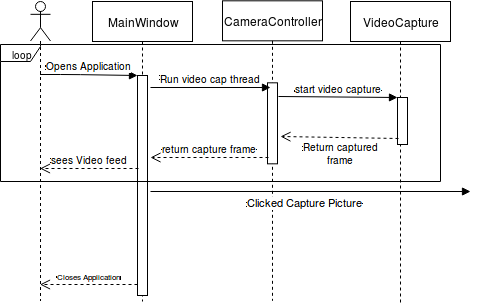
\includegraphics[width=0.5\textwidth]{SD_video_feed.png}
    \caption{Displays the sequence that is taken to display the video feed at the start of the application. The sequence diagram shows that the MainWindow will go into a continuous loop of talking to the Camera and VideoCapture class to get frames to display on the GUI as the video capture. When the Capture Image button is pressed by the user, then the GUI will move onto the next page asking if the captured image is suitable for what the user wants.}
    \label{fig:SD_video_feed}
\end{figure}
\begin{figure}[h]
    \centering
    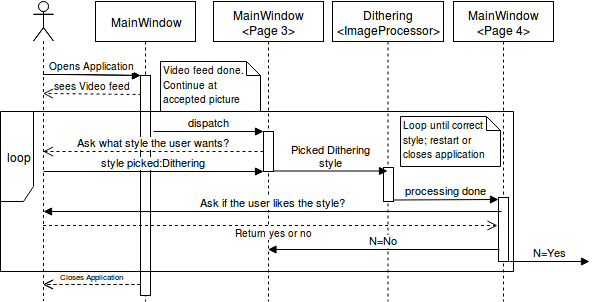
\includegraphics[width=0.65\textwidth]{SD_Image_Processing.png}
    \caption{Displays the sequence that is taken to process an Image. This is after the sequence of events in Figure \ref{fig:SD_video_feed} and the Image has been accepted to be processed. The user will be taken to page 3 of the GUI. This is the style selection page. After one style has been selected the image will be processed for the specified style. In this case, it is the Dithering style. So the program will run the method run() in the image processor Dithing.py. After this the finalized style will be displayed on page 4. Then there are two sequences of events either the user can accept the style and start the plot or reject the style and go back to page 3.}
    \label{fig:SD_image_processing}
\end{figure}
\begin{figure}[h]
    \centering
    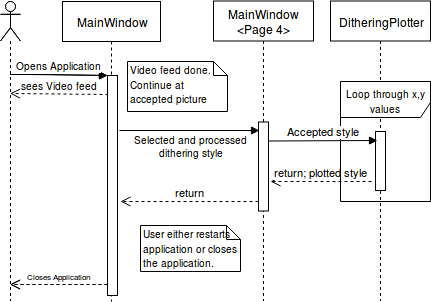
\includegraphics[width=0.45\textwidth]{SD_Plotting.png}
    \caption{Displays the sequence that is taken to plot the style that was processed through the given style. This involves when the style has been accepted on page 4, as continued from Figure \ref{fig:SD_image_processing}. Then the coordinates are gathered from that style in the MainWindow class, then the thread for plotting that specified style begins. This involves sending multiple HPGL commands through serial communication to the plotter. After this task is plotted and all coordinates that were made are complete then the application is restarted from the beginning or the application is closed.}
    \label{fig:SD_plotting}
\end{figure}
\clearpage
    \section{Graphical Unit Interface(GUI) Design}
This section will discuss the interface design that was developed for the project. The design was developed for python 2.7 using the library PYQT 4\cite{pyqt}. The overall development was done using the software called 'QT Designer'\cite{qt_designer}. This allowed the project to save time as the GUI didn't take as much time to develop. The project being developed can be seen in Figure \ref{fig:Qt_designer}.

Figures \ref{fig:page_1}, \ref{fig:page_2}, \ref{fig:page_3} and \ref{fig:page_4} show the design of the overall GUI. From pages one to four in respective order. These designs were all made with QT Designer and then the actions and code were added to the MainWindow class that can be seen in Figure \ref{fig:class_diagram}.
\\ \newline
The design also has a description of what the project is about on the left-hand side of the GUI. This is a label that takes text from the description.txt file that can be found in the code folder. \\ \newline
\begin{figure}[h]
    \centering
    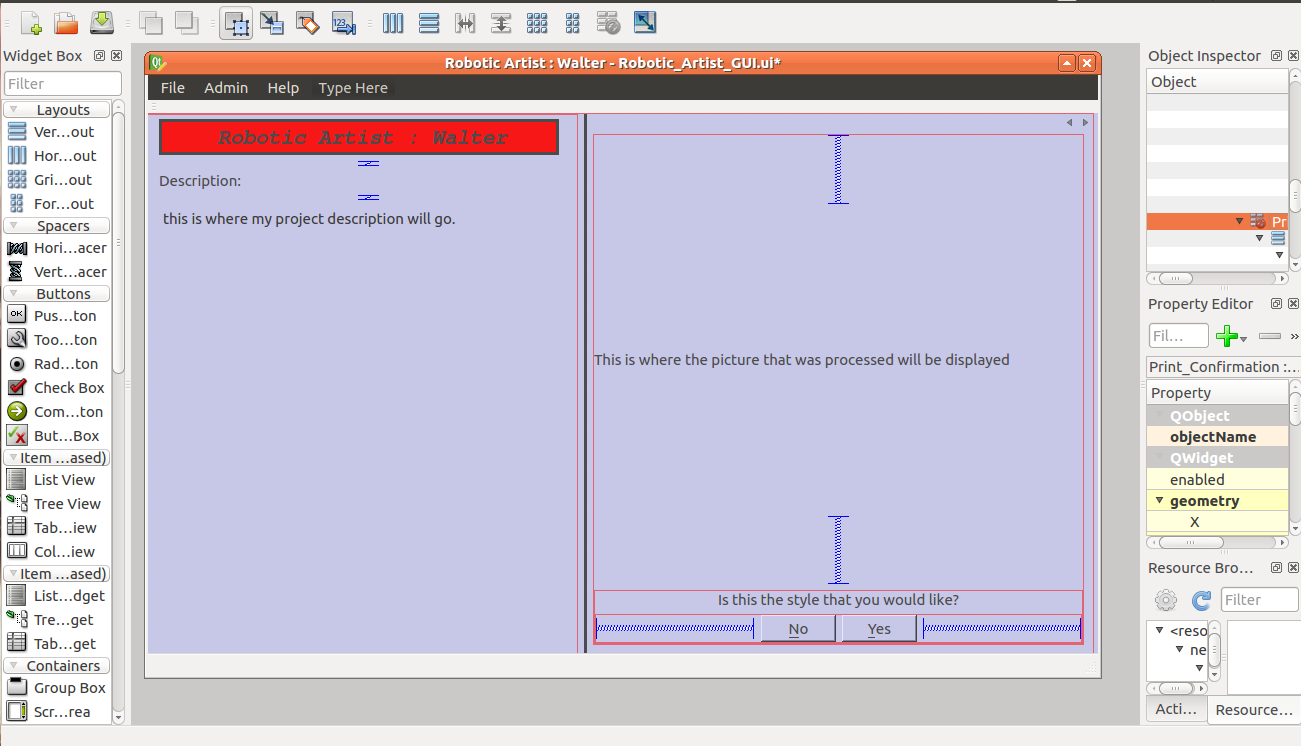
\includegraphics[width=0.65\textwidth]{qt_designer.png}
    \caption{This is an example of how the QT designer software looked when developing the GUI for the project}
    \label{fig:Qt_designer}
\end{figure}

\begin{figure}[h]
    \centering
    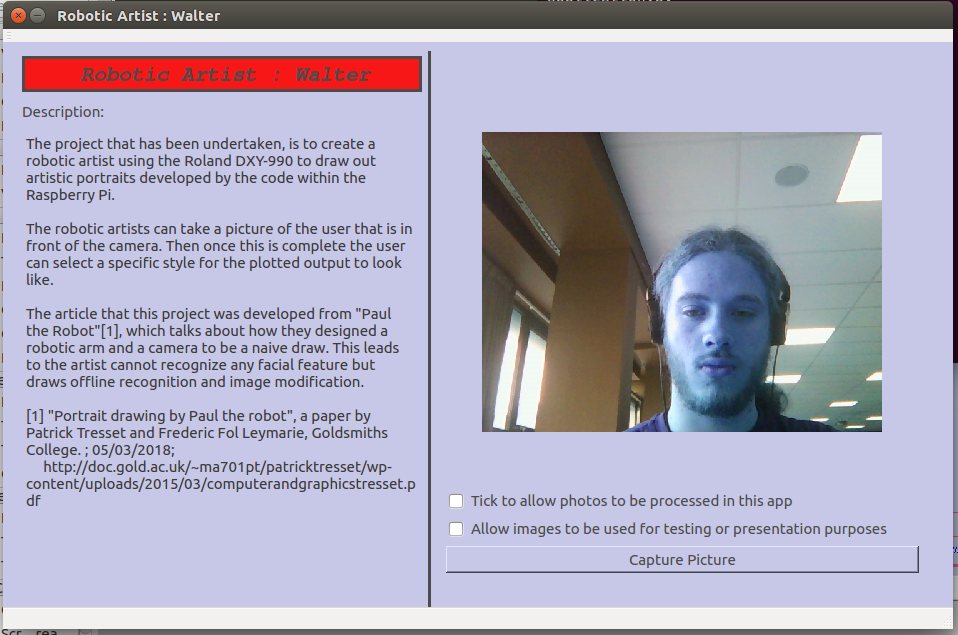
\includegraphics[width=0.65\textwidth]{page1.png}
    \caption{Page 1: Video capture. This page was designed to contain the video capture from the camera. The design of the page is to have a label that a QImage can be added to. During runtime, the image will continuously be updated through a QThread. The other parts of the page are two checkboxes and a button at the bottom of the page, which stops the video capture and take the frame it was on as a picture. This routine can be seen in Figure \ref{fig:SD_video_feed}.}
    \label{fig:page_1}
\end{figure}

\begin{figure}[h]
    \centering
    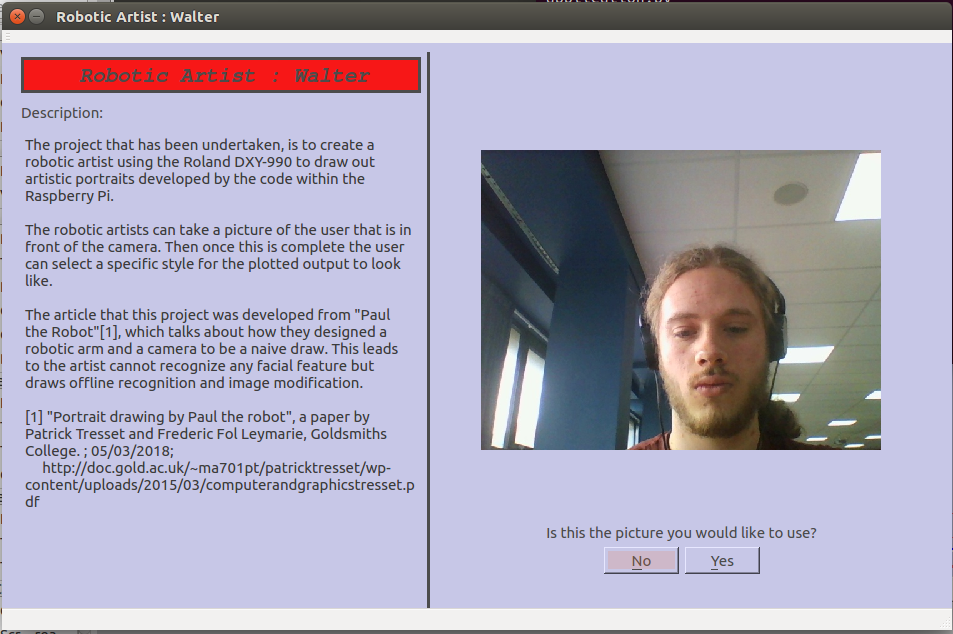
\includegraphics[width=0.65\textwidth]{page2.png}
    \caption{Page 2: Picture Acceptence. This page has a label that will contain the captured frame. Then there are a set of buttons that ask yes or no to whether the picture taken is correct.}
    \label{fig:page_2}
\end{figure}

\begin{figure}[h]
    \centering
    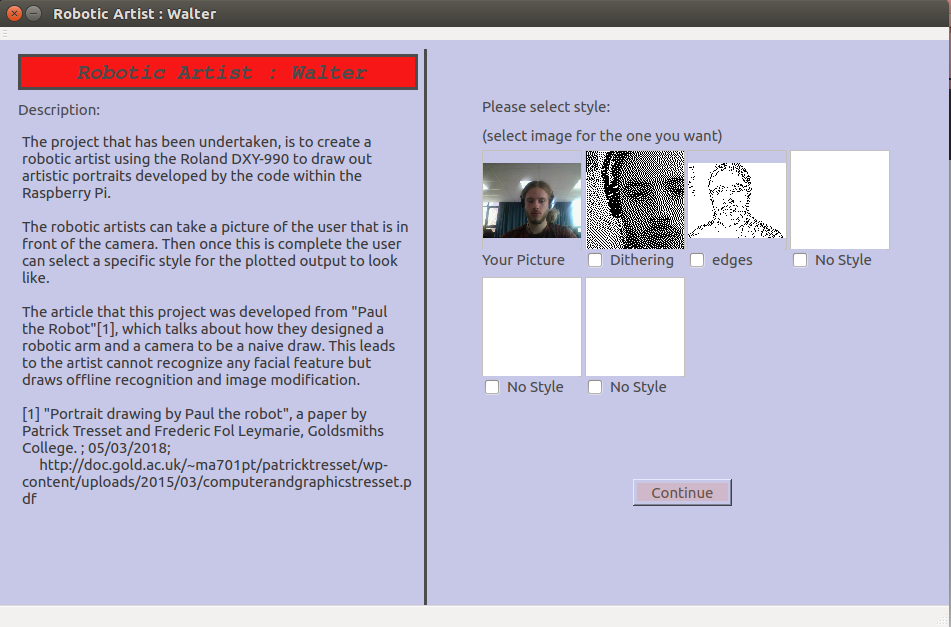
\includegraphics[width=0.65\textwidth]{page3.png}
    \caption{Page 3: Style selection. This page is all about selecting the individual style you want. There is a grid layout with labels inside them that display either text or images. These make a grid that displays the styles image and the name of each of the styles. In this section, you are only allowed to select one style. Then once you have selected that style and pressed the button the program will process the image from the style that you have selected. At the moment the GUI has a limit of 5 styles to pick from when they are all made. However, modification to the code will allow more in line with additional styles being developed.}
    \label{fig:page_3}
\end{figure}

\begin{figure}[h]
    \centering
    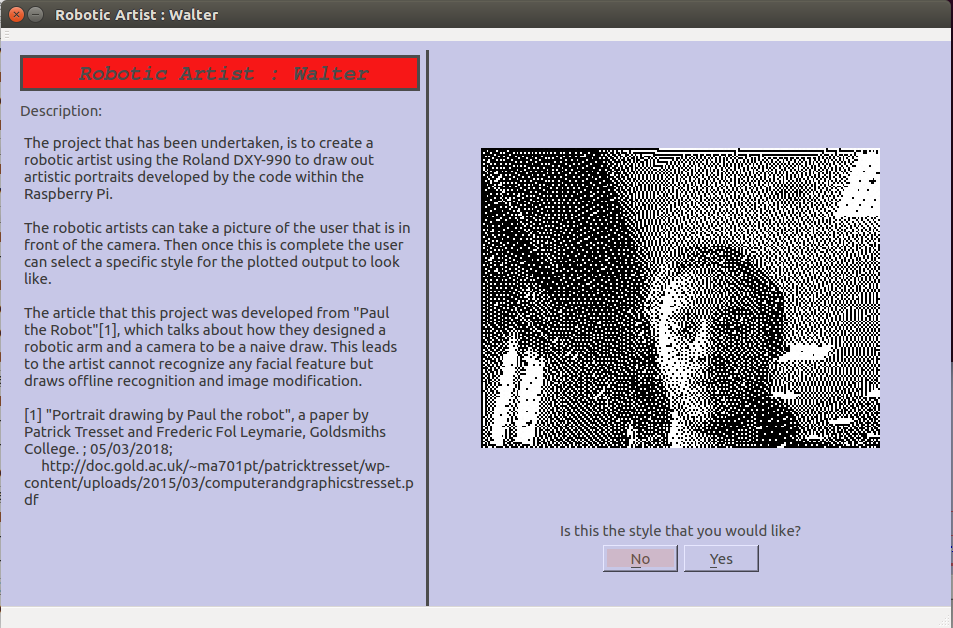
\includegraphics[width=0.65\textwidth]{page4.png}
    \caption{Page 4: Style confirmation. This page has a label that contains the stylized image and then a button at the end of the page that allows the user to accept or reject the style.}
    \label{fig:page_4}
\end{figure}

\clearpage
    \section{Versions}


\begin{center}

\begin{tabular}{| l | p{8cm} | p{3cm}|}

\hline

\textbf{Version} & \textbf{Description} & \textbf{Date Modified} \\\hline

0.1 & created basic structure for introduction and version control. Added sequence diagrams and class diagram. & 23/04/2018 \\ \hline
0.2 & wrote the content for the UML diagram. As well, added to the section to the GUI design section. & 25/04/2018\\ \hline
0.3 & proofread and corrected the document. As well, added reference when required to the document.& 26/04/2018\\ \hline
0.3.1 & made minor corrects; changed page 4 to style confirmation from style acception & 27/04/18 \\ \hline
\end{tabular}

    \begin{thebibliography}{9}

    \bibitem{Requirement_specifications}

    Matthew Howard (mah60);Requirement Specifications; 25/04/2018 \\ 
    
    This document talks about the requirements that have been given to robotic artist project. The document can be found in the Appendices for this project.\\ 
    
    \bibitem{qt_designer}

    QT Documentation;QT Designer Manual; 26/04/2018 \\ 
    
    \textit{http://doc.qt.io/qt-5/qtdesigner-manual.html}
    
    This site is a manual on how to use the Qt Designer software and demonstrates the software that was used to develop the GUI in this project.\\ 
    
    \bibitem{pyqt}

    Python Wiki;Pyqt4 library; 26/04/2018 \\ 
    
    \textit{https://wiki.python.org/moin/PyQt4}
    
    This site talks about the pyqt library that I used to develop the GUI. As well, provides learning materials to understand the library.\\ 
    

    \end{thebibliography}

\end{center}

 \end{document}